%!TEX ROOT=ctutest.tex
\chapter{HW Specification}
    This chapter serves as a description of hardware components used in the system. Attention will be given to the technical details of specific components and the reasons behind choosing them.
    
\section{HW of Light Control Unit}
    The light control unit board is based on the nRF52833 BLE SOC (System on Chip) from Nordic Semiconductor. The board also contains a stabilizer circuit, charger circuit, USB-C connector, three small RGB LEDs for signalization and one push button.\\
    Another part is a step-up converter based on the DIO5661 chip with SEPIC (Single-ended Primary-inductor Converter). This PWM to constant current converter controls the electrical current in optic fibres - the board is connected to them through 2.5 mm jack.
    
    Finally, the board also contains an accelerometer/gyro LSM6DSMTR and a microphone. 
    The 1600mAh 3.7V Lithium-ion rechargeable battery is soldered directly on the PCB and needs to be connected with a jumper. To increase the reach, a Molex 2.4/5 GHz antenna can be connected as well. 

    \subsection{Microcontroller (MCU)}
        The nRF52833 is general-purpose multi-protocol SOC (System On Chip) device supporting not only BLE but also Zigbee, Bluetooth Mesh and NFC.
        
        \begin{figure} [!hb]
    	    \centering
    	    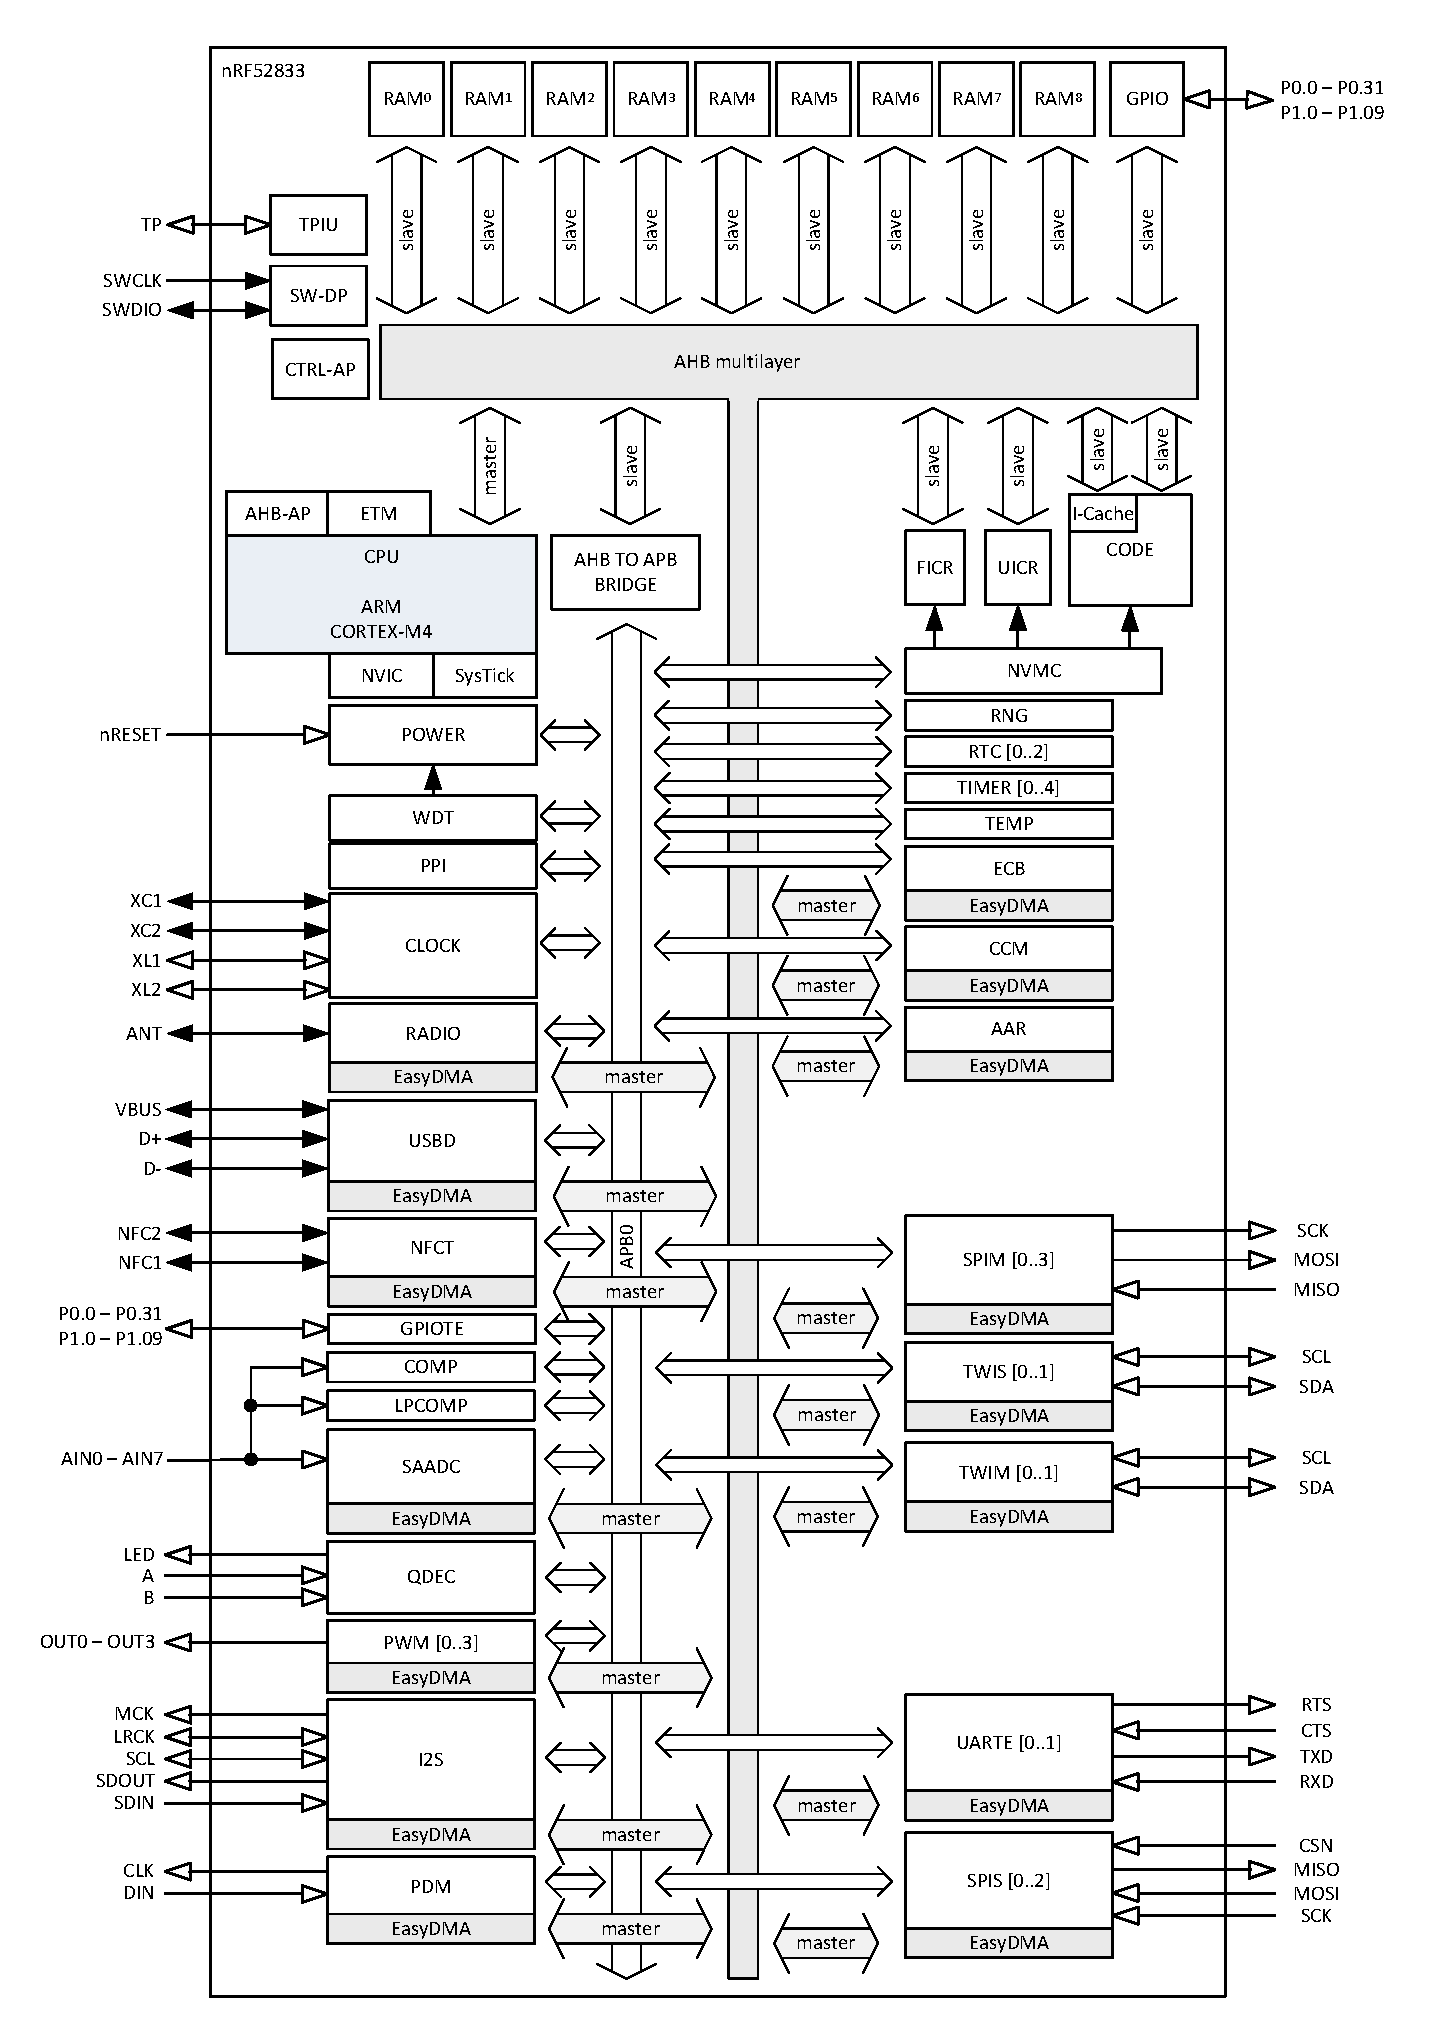
\includegraphics[ width =0.8\textwidth]{02.HW/Figs/nrf52833_blockdiagram.pdf}
            \caption {nRF52833 block diagram (taken from \cite{image:nrf52833_block_diagram})}
        \end{figure} 
        
        
        \begin{titleitemize}{Specification of nRF52833 with selected peripherals:}
            \item 32-bit RISC ARM Cotex M4 with FPU, 64 MHz 
            \item 512 kB flash and 128 kB RAM memory 
            \item HFCLK from 64 MHz on-chip oscillator / 32 MHz external oscillator, LFCLK from 32 kHz RC oscillator 
            \item 42 GPIO pins
            \item 12-bit ADC 200 ksps, 8 channels 
            \item 4x PWM, 4 channels
            \item 2x UART, 4x SPI, 2x $\text{I}^2\text{C}$
            \item 5x 32-bit timer with counter mode, 3x RTC counter
            \item temperature sensor
        \end{titleitemize}
        \newpage    
        
            \begin{titleitemize}{Power Management:}
                \item Power consumption in SYS-OFF mode:  \SI{0.6}{\micro\ampere} (at 3V)
                \item Power consumption in SYS-ON mode (IDLE):   \SI{1.5}{\micro\ampere} (at 3V)
                \item 4.9 mA peak current in TX (0 dBm)
                \item 4.6 mA peak current in RX
            \end{titleitemize}
        
        
        \subsubsection{PPI}
        \label{sec:ppi}
             PPI (Programmable Peripheral Interconnect) is an advanced chip's interface that allows peripherals to connect and communicate with each other using a system of tasks and events without the need of the MCU. It becomes beneficial especially when precise synchronization between events and tasks is needed (for example, sampling).
        
        \subsubsection{EasyDMA}
            EasyDMA is easy to use Direct Memory Access that provides some peripherals with direct access to the RAM without the need of the MCU. Multiple DMA instances for a peripheral are allowed, so writing to the RAM and reading from it is possible simultaneously.
        
        
        \subsubsection{ADC}
            The successive approximation analog-to-digital converter supports up to eight external input channels (8 single-ended inputs or 4 differential inputs) in 8/10/12 bit resolution.
            
            Each ADC channel can use an individual voltage reference - either the 0.6 V internal reference or VDD/4. Using the VDD based reference is useful if the measured signal fluctuates depending on VDD.
            
            The maximum sampling frequency is 200 kHz (inverse value of summation of conversion time - $t_{conv} = \SI{2}{\micro\second}$ and minimum acquisition time - $t_{acq} = \SI{3}{\micro\second}$. The acquisition (sampling) time determines how long the channel input is connected to the external source. 
            
            % The simplified scheme of nRF52 ADC:
                
    \subsection{Radio}
        The 2.4 GHz transceiver is integrated on the nRF52833 chip. It supports multiple radio standards such as 1/2 Mbps BLE modes, long range 250/500 kbps BLE modes or IEEE 802.15.4 based 250 kbps mode (LR-WPAN). Besides that, it also implements the Bluetooth direction finding.
        
        The radio uses DMA for reading and writing data packets from and to the RAM without CPU involvement. Apart from that, it involves an automated packet assembler, packet disassembler, automated CRC generator and CRC checker.
        
        % \textbf{Specification of radio:}
            \begin{titleitemize}{Specification of radio:}
                \item 1 and 2 Mbps BLE modes
                \item 250 and 500 kbps long range BLE modes 
                \item IEEE 802.15.4 250 kbps mode (LR-WPAN)
                \item -96 dBm sensitivity in 1 Mbps BLE mode
                \item -103 dBm sensitivity in 125 kbps BLE mode (long range)
                \item -20 to +8 dBm TX power, configurable in 4 dB steps
            \end{titleitemize}
            
            \begin{figure} [!ht]
        	    \centering
        	    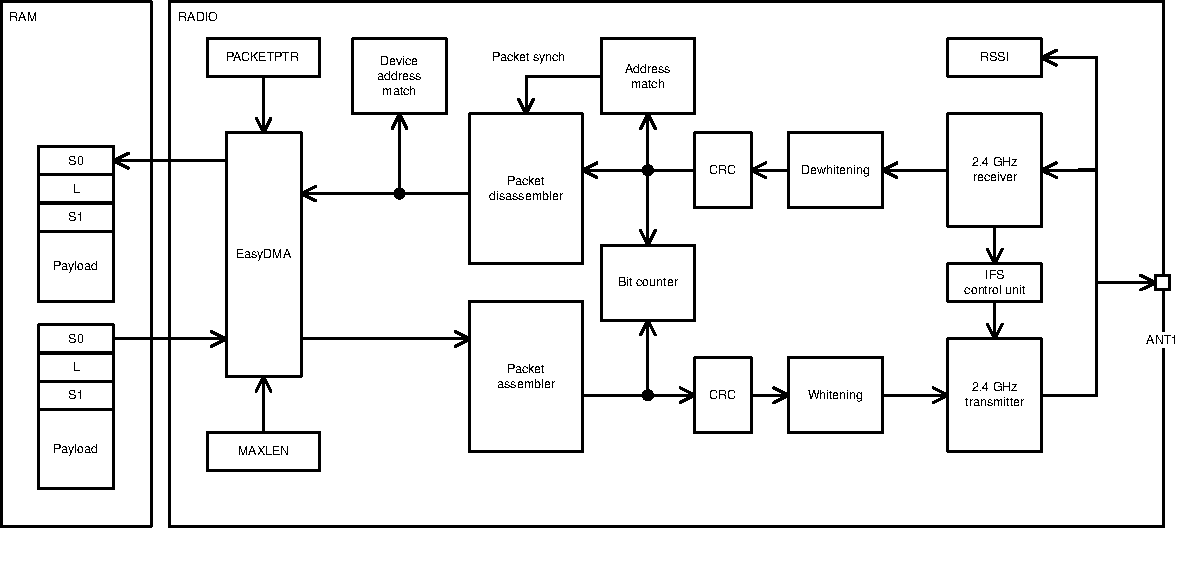
\includegraphics[ width =1.05\textwidth]{02.HW/Figs/nrf52833_radio.pdf}
                \caption {nRF52833 radio block diagram (taken from \cite{image:nrf52833_radio_block_diagram})}
            \end{figure} 
                

     
    \subsection{Gyroscope/Accelerometer}
        \todo{TO BE DONE ...}
        
        % The choice of LSM6DSMTR accelerometer/gyro was determined mostly by...
        % \textbf{Specification:}
    
    % \subsection{SEPIC}
        
        %     \todo{Provide some theoretical background/calculations to SEPIC circuit}
    
    
    \subsection{The Overall Design}
        The first version of the hardware of the light control unit was designed by Pavel Porazil from PiKRON company during summer 2021. The case for the unit and the sticker comes from SCILIF company directly.
        
        \begin{figure} [!ht]
    	    \centering
    	    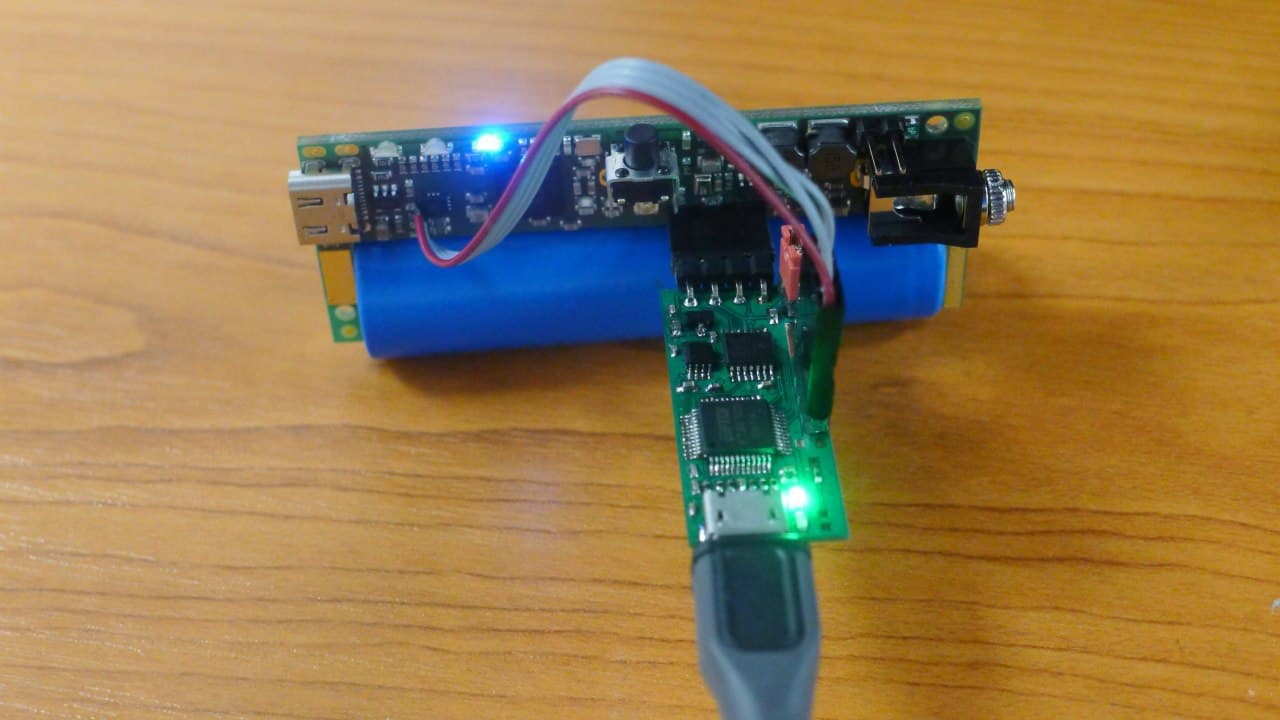
\includegraphics[ width =0.8\textwidth]{02.HW/Figs/overall_unit.jpg}
            \caption {Light Control Unit board from Pavel Porazil with PiKRON programmer}
        \end{figure} 
    
\section{HW of Floating Button}
    For the first prototype of the floating button, the development board BBC micro:bit.v2 was selected. The fact that the board is based on the nRF52833 as well helped significantly during programming.
    
    The board also comprises LED matrix of 25 LEDs, two push buttons, a micro-USB connector, two signalization LEDs, a microphone, speaker, touch sensor and accelerometer/magnetometer LSM303AGRTR. 
    
        \begin{figure} [!ht]
            \centering
            \caption{BBC micro:bit.v2 (taken from \cite{image:BBC_microbit})}
            \begin{subfigure}[b]{0.48\textwidth}
                 \centering
                 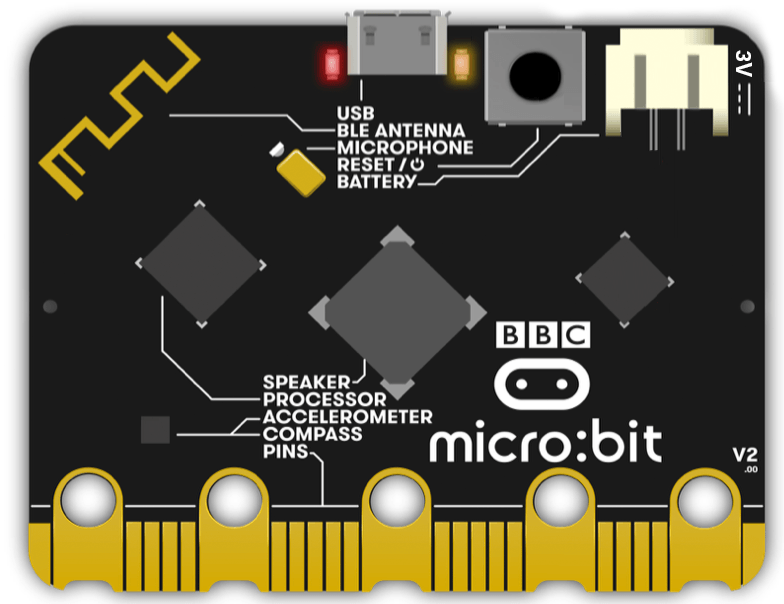
\includegraphics[width=\textwidth]{02.HW/Figs/microbit.png}
             \end{subfigure}
             \hfill
            \begin{subfigure}[b]{0.45\textwidth}
                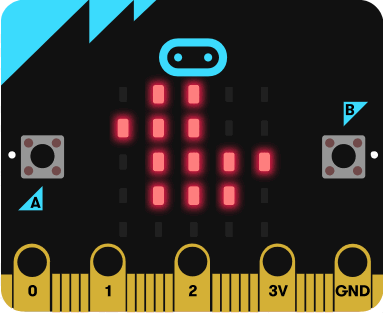
\includegraphics[width=\textwidth]{02.HW/Figs/microbit3.png}
            \end{subfigure}
        \end{figure}     
        
    \subsection{Accelerometer/Magnetometer}
        \todo{TO BE DONE...}
        % \textbf{Specification:}


\section{HW of RFID Switch}
    \label{sec:hw_rfid_switch}
     The RFID switch consists of an active reader and a passive tag. The RFID reader can be integrated as a part of the light control unit board or connected and powered externally. In both cases, the coil (antenna) must be wired to the reader. 
    
    \subsection{RDM6300 RFID Reader}
        \label{sec:hw_rfid_rdm6300}
        As a first prototype of the RFID reader, the development module RDM6300 was chosen. RDM6300 is a LF RFID reader designed to read data from 125 kHz, EM4100 compatible tags using a RF receiver circuit and built-in MCU. An external antenna needs to be connected to the board directly.
        The RDM6300 uses demodulation and decoding algorithms and only transmits the received bits over a serial communication (UART) at a 9600 baud rate.\\
        The whole module was connected to the light control unit through a few jumper wires.
        
        
        % \textbf{Specification of RDM6300:}
        \begin{titleitemize}{Specification of RDM6300:}
            \item 125 kHz operating frequency 
            \item 20-50 mm receive distance
            \item around 50 mA working current
            \item 5V working voltage
        \end{titleitemize}
            
        \begin{figure} [!ht]
            \centering
            \caption{EM4100 RFID tag and RDM6300 RFID reader (taken from \cite{image:em4100}, \cite{image:rdm6300})}
    
            \begin{subfigure}[b]{0.45\textwidth}
                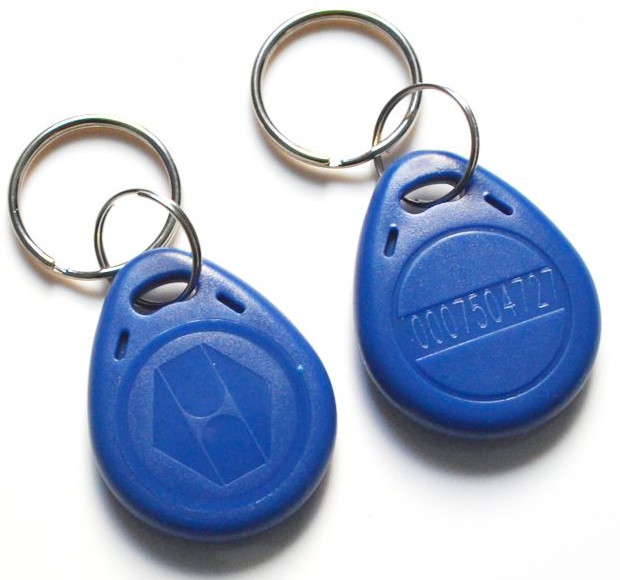
\includegraphics[width=\textwidth]{02.HW/Figs/em4100.jpg}
            \end{subfigure}
             \hfill
            \begin{subfigure}[b]{0.45\textwidth}
                 \centering
                 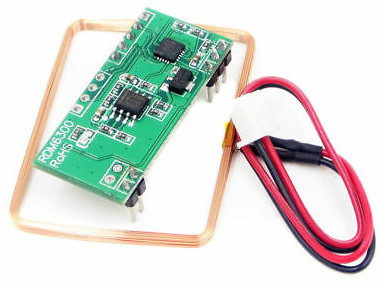
\includegraphics[width=\textwidth]{02.HW/Figs/rdm6300.jpg}
             \end{subfigure}
        \end{figure}     
             
        
            
    \subsection{Custom Low Power RFID Reader}
        The main drawback of the RFID reader lies in a high standby current consumption (around 50 mA). A custom low power RFID reader circuit was designed to mitigate this problem \ldots
        
        \todo{TO BE DONE...}
        
    \subsection{EM4100 RFID Tag}
        The RFID tag in a key fob form is based on a cheap EM4100 chip made by the company EM Microelectronic. 
        The 64 bits of data are read-only, factory preprogrammed,  and represent a unique identifier of the tag, which is also printed on the PVC, so it can not be changed. \\
        The RFID reader must know how the data is stored in the tag and which protocol to use to extract it - demodulation and decoding method.
        

% \section{Additional Fast thoughts}
%     The solution has been use only with specific SCILIFF


\todo{Include analyisis of current BLE based MCUs}

\todo{Provide some theoretical background to SEPIC}


